%\documentclass[sigconf]{acmart}
\documentclass[sigconf, 10pt]{acmart}
\usepackage{graphicx}
\graphicspath{ {./images/} }

% Copyright
% Pick the correct copyright notice that matches your rights form
%\setcopyright{none}
\setcopyright{acmcopyright}
%\setcopyright{acmlicensed}
%\setcopyright{rightsretained}
%\setcopyright{usgov}
%\setcopyright{usgovmixed}
%\setcopyright{cagov}
%\setcopyright{cagovmixed}

% DOI
%\acmDOI{10.475/1234.5678}

% ISBN
%\acmISBN{123-4567-24-567/08/06}

%Conference
\acmConference[SYSTOR'21]{ACM International Systems and Storage Conference}{June 14-16, 2021}{Haifa, Israel}
\acmYear{2021}
\copyrightyear{2021}

%\acmArticle{4}
\acmPrice{15.00}

% These commands are optional
%\acmBooktitle{Proccedings of the ACM International Systems and Storage Conference}
%\editor{John Doe}
%\editor{Jane Doe}

\begin{document}

\title{CRDTs for truly concurrent file systems}

% Fill in your details. The \documentclass "anonymous" parameter keeps them hidden, remove it after the review process finishes
\author{Romain Vaillant}
\affiliation{%
  \institution{Scality}
  \city{Paris}
  \country{France}
}
\email{romain.vaillant@scality.com}

\author{Dimitrios Vasilas}
\affiliation{%
  \institution{Lip6}
  \city{Paris}
  \country{France}
}
\email{dimitrios.vasilas@lip6.fr}

\author{Marc Shapiro}
\affiliation{%
	\institution{Inria \& Lip6}
	\city{Paris}
	\country{France}
}
\email{marc.shapiro@acm.org}

\author{Linh Thuy}
\affiliation{%
	\institution{Grenoble University}
	\city{Grenobnle}
	\country{France}
}
\email{thuy-linh.nguyen@univ-grenoble-alpes.fr}

% The default list of authors is too long for headers.
\renewcommand{\shortauthors}{R. Vaillant et al.}

\begin{abstract}

Building scalable and highly available geo-replicated file
systems is hard. These systems need to resolve conflicts that
emerge in concurrent operations in a way that maintains
file system invariants, is meaningful to the user, and does
not depart from the traditional file system interface. Conflict
resolution in existing systems often leads to unexpected
or inconsistent results. This paper introduces ElmerFS, a
geo-replicated, truly concurrent file system designed with
the aim of addressing these challenges. ElmerFS is based
on two key ideas: (1) the use of Conflict-Free Replicated
Data Types (CRDTs) for representing file system structures,
which ensures that replicas converge to a correct state, and
(2) conflict resolution rules, which are determined by the
choice of CRDT types and their composition, are designed
with the principle of being intuitive to the user. We argue
that if the state of the file system after resolving a conflict
conveys to the user the resolved conflict in an intuitive way,
the user can complement or reverse it using traditional file
system operations. We discuss the challenges in the design
of geo-replicated weakly consistent file systems, and present
the design of ElmerFS.

\end{abstract}

%% Note: Classification and Keywords are only required for the camera-ready version

%
% The code below should be generated by the tool at
% http://dl.acm.org/ccs.cfm
% Please copy and paste the code instead of the example below.
%
\begin{CCSXML}
	<ccs2012>
	   <concept>
		   <concept_id>10010520.10010575.10010755</concept_id>
		   <concept_desc>Computer systems organization~Redundancy</concept_desc>
		   <concept_significance>500</concept_significance>
		   </concept>
	   <concept>
		   <concept_id>10011007.10011074.10011075.10011077</concept_id>
		   <concept_desc>Software and its engineering~Software design engineering</concept_desc>
		   <concept_significance>300</concept_significance>
		   </concept>
	   <concept>
		   <concept_id>10011007.10011074.10011075.10011077</concept_id>
		   <concept_desc>Software and its engineering~Software design engineering</concept_desc>
		   <concept_significance>300</concept_significance>
		   </concept>
	   <concept>
		   <concept_id>10010520.10010521.10010537.10010538</concept_id>
		   <concept_desc>Computer systems organization~Client-server architectures</concept_desc>
		   <concept_significance>300</concept_significance>
		   </concept>
	   <concept>
		   <concept_id>10010520.10010575.10010578</concept_id>
		   <concept_desc>Computer systems organization~Availability</concept_desc>
		   <concept_significance>500</concept_significance>
		   </concept>
	   <concept>
		   <concept_id>10010520.10010575.10010577</concept_id>
		   <concept_desc>Computer systems organization~Reliability</concept_desc>
		   <concept_significance>500</concept_significance>
		   </concept>
	 </ccs2012>
\end{CCSXML}

\ccsdesc[500]{Computer systems organization~Redundancy}
\ccsdesc[300]{Software and its engineering~Software design engineering}
\ccsdesc[300]{Software and its engineering~Software design engineering}
\ccsdesc[300]{Computer systems organization~Client-server architectures}
\ccsdesc[500]{Computer systems organization~Availability}
\ccsdesc[500]{Computer systems organization~Reliability}

% \keywords{ACM proceedings, \LaTeX, text tagging}

\maketitle

\sloppy

\section{Introduction}

File systems services are essential for data sharing and collaboration among users.
These services must provide low response time, remain available in the presence
of network partitions, and provide support for offline work \cite{howard1988scale}.
To achieve these goals, these services typically replicate
data among geographically distant sites and serve each user request from the replica
closer to the user, without coordination with other replicas.

This type of design allows replicas to accept concurrent operations that conflict
with one another, for example concurrently creating two files with the same name
under the same directory on two different replicas.
As a result, these systems face two challenges:
resolving conflicts between concurrent operations in a way that is meaningful to the users while maintaining file system invariants,
and ensuring support for legacy applications and protocols that have not been developed with mechanisms for dealing with concurrency anomalies and are still widely in use.

It has been shown that existing file system services that support collaboration
and offline work resolve some conflicts in inconsistent, non-deterministic or unexpected ways \cite{cai2018some, taothanh:tel-01673030}.
For example, in Google Drive the conflict described above can result in replicas presenting different views of the file system.

This makes it difficult for users to have an intuitive understanding about
the behaviors of these services,
leading to misconceptions on their expected behavior~\cite{tang2013you}.

A solution to that could involve more flexible conflict resolution mechanisms,
for example requiring user input in the process of conflict resolution.
However, enabling such functionality while maintaining support for legacy applications
through POSIX compliance is challenging.

In this paper, we present a comprehensive analysis of the challenges in
the design of geo-replicated weakly consistent file systems.
Guided by this analysis, we introduce ElmerFS,
a geo-replicated file system that provides intuitive conflict resolution
semantics, while maintaining support for legacy applications.
The design of ElmerFS leverages the properties of Conflict-Free Replicated Data Types (CRDTs) to ensure that concurrent operations on different replicas always converge to a correct state while preserving the semantics of a traditional POSIX file system.
The guiding principle for designing conflict resolution in ElmerFS is that
it should be intuitive to the user and minimally disruptive for applications.
This is achieved by designing conflict resolution rules that
(1) preserve the effects of conflicting operations as much as possible,
and (2) do not introduce changes not explicitly expressed by the conflicting operations.

\section{Related Work}

Designing a geos-distributed file system using CRDTs is not a novel idea, "Merging semantics for conflict updates in geo-distributed file systems"\cite{tao2015merging} categorizes various conflicts in a weakly-consistent file system and describes how it could be designed as one CRDT that solve conflicts in a precise manner.
However, while it provides a good description on how such system could be designed, it misses a practical approach to the problem. When using existing, formally proven CRDTs, keeping the application invariant is often not straight-forward.

Closely related to our work, "File System on CRDT"\cite{ahmed2012file} is a description of simplified file system based on CRDTs which solve conflicts with multiple correction layers and by building a view of the underlying system. Their solutions use renaming for name conflict and after-the-fact automatic conflict resolutions, a design from which we want to depart to support legacy application and to help users to build a simple mental model of the underlying system.



\section{Designing a file system}

\subsection{File systems under weak consistency}
\label{fs:weak}

Preserving file system invariants in a replicated file system
that allows updates in multiple replicas with coordination
among them presents several challenges:

\begin{itemize}
	\item \textbf{Unique identifiers}: Any operation that creates
	inodes needs to generate a unique identifier.
	Without coordination among replicas, generated ids might conflict.
	In practice, this is addressed using 16 byte ids.
	However, this is not compatible with the POSIX specification, which requires 8 byte ids.
	\item \textbf{Named links}: Operations that create or move objects (files or directories)
	may result in conflicts in which concurrent operations on different replicas create
	objects with the same name in the same directory.
	Existing systems resolve naming conflicts between files by automatically renaming
  files, and conflicts between directories either by renaming or by merging them.
    \item \textbf{Cycles}: Concurrent move operations without coordination may violate the file system invariant.
    For example, merging an operation that moves a directory A into a
	directory B with a concurrent operation that moves B into A can result in a cycle.
    Merging two concurrent operations that move the same directory to different destinations can result in a directory with two parents.
  \item \textbf{Divergent renames}: The \textit{rename} operation is semantically a move operation, it move a link from one folder to another. When two concurrent renames move the same link to two different places, if both rename are ultimately accepted, a additional link of the inode will be created. The file system must ensure that the number of link of a inode is always correctly tracked.
  \item \textbf{Deletion of inode}: When operations can be concurrent with the deletion of an inode, the file system
  must ensure that either the deletion is cancelled and the inode restored or that the deletion is kept honored.
  \item \textbf{Permissions changes}: Updating permission from a replica may take some time to be enforced in other replicas.
  Merging an operation that removes a Bob's permission to write to file with a concurrent operation in which Bob writes
  to that file will result in a different outcome depending on the order in which operations are applied.
  % (This is very interesting but can create a lot of questions, it's maybe better to avoid mentioning permissions)
\end{itemize}

\subsection{Assumptions and objectives}

We leverage CRDTs to develop a file system that is always available
and that provides good response times whatever the network conditions.
It must support active/active configurations
(i.e. two geographically distant clusters can issue read, write and structural
operation at the same time without coordination with each other).

The behavior of the file system should remain as close as possible to a local file system.
In summary, we want the following properties:

\begin{itemize}
	\item \textbf{Preserve intention}: We minimize changes not explicitly requested by the user.
	The user should to be able to develop a simple mental model to understand
	the underlying convergence properties.
	\item \textbf{Truly concurrent operations}: The FS should be always available even under extreme network conditions.
	One way to handle concurrency
	is to use consensus to serialize operations applied on the relevant objects.
	CRDTs avoid this and allow true concurrency without the need for a consensus.
	\item \textbf{Follow the POSIX standard}: Legacy protocols and a wide range of user applications expect some strong invariants on their file system. Often more than what POSIX describes. We follow this standard to explore the flexibility of using CRDTs on systems which rely on strong invariants.
	\item \textbf{Atomic operation}: No matter how complex a FS operation is, it should be either performed or completely discarded.
	\item \textbf{Active-Active}: Several replicas accept operations
	(structural and updates) concurrently and propagate them from one-another,
	even after long delays.
\end{itemize}

Our focus therefore is to leverage CRDTs to create a highly resilient and
truly concurrent file system that follows the strict POSIX invariants
while providing users a simple interface to deal with conflicting updates.

\section{System Overview}

\subsection{Modeling the file system using CRDTs}

Ensuring that all replicas converge to the same state without coordination
is not trivial.

Conflict-Free Replicated Data Types (CRDTs) are data structures that
can be replicated across multiple replicas,
and these replicas can be updated independently and concurrently without coordination~\cite{shapiro2011conflict}.fo

By construction, CRDTs guarantee that modifications on different
replicas can always be merged into a consistent state without requiring
any special conflict resolution code or user intervention.

Moreover, the rules used for conflict resolution are parts of each CRDT's definition.
Therefore, application developers can control their conflict resolution semantics by
choosing the types of CRTDs they model their application with.

ElmerFS uses the following CRDT types provided by AntidoteDB~\cite{akkoorath2016antidote, akkoorath2016cure}, a CRDT key-value store:

\begin{itemize}
	\item \textbf{Remove Win Map} (RWMap): A RWMap is a map data type that associate an arbitrary key to a CRDT value, The Remove Win semantic arbitrates conflicting add and remove operations in favor of the remove.
	\item \textbf{Remove Win Set} (RWSet): A set data structure containing LWWRs. It has add and
    remove operations. As with the RWMAP, it favors remove operations in conflicting situations.
	\item \textbf{Last Writer Win Register} (LWWR): A LWWR can be viewed as a blob of data that retains only the last applied update.
    For concurrent updates, a mechanism based on replica identifiers and timestamps, ensures that the same retained across all replicas.
\end{itemize}

ElmerFS represents the state of the file system using CRDTs.
The four main entities are inode objects, symbolic links, blocks and directories.
An inode structure stores metadata for an inode in the file system. using a Remove Wins Map

We represent a file as a collection of fixed-size blocks. Each block is represented using a LWWR. Blocks have a fixed size, they can be addressed with the concatenation of an offset and an ino.
We do not keep track of the allocated block of a file, we rely on the file size to recover this information. This is simplistic design that might lead to mixing file content if multiple applications updates are not aligned on the block size and this assumes that nodes have a synchronized clock which is not easily achievable. Further work needs to be done for allowing file content to diverge without loss of data or to use a CRDT that would be appropriate for a given file format.

We represent a symbolic link as a special case of a file, storing exclusively the target path.

We represent a directory using a Remove Win Set (RWSet), a set data type with semantics similar to the RWMap. Directory entries in the set are inode number - name pairs. Directory contains its child directories, a child directory keeps a pointer to its parent through the special ".." named file.

%Ideally a RWMap whose keys are file names would have been a better choice, however AntidoteDB doesn't support querying specific fields of a map, we had to resort to using a RWSet but we considered two directory entry to be equal if their name are equal as any more practical implementation will want to
%be able to lookup entries with the parent inode number and the name without loading the whole folder in memory.

The design decision of choosing the Remove Win semantic instead of its Add Win counterpart is discussed in Section~\ref{sec:deletion}.

\subsection{The layered architecture of ElmerFS}

An ElmerFS deployment consists of a number of data centers.
Each data center holds a full replica of the file system.
Clients communicate with the data center nearest to them.
Every operation is served by the local data center, without the need
for coordination across data centers,
and updates are asynchronously propagated between data centers.
A data center continues serving user requests even if connectivity
with other data centers is lost due to network partitions.

Within a data center, an ElmerFS cluster consists of an arbitrary number
of node and a shared-nothing architecture.

An ElmerFS node is a daemon consisting of the following layers.

\subsubsection{Interface}

The interface layer is responsible for handling interaction between the client applications
and the file system.

It is based on the FUSE protocol, a user-space protocol used to implement
file systems. The interface layer receives a FUSE request, calls the corresponding operation in the translation layer(\S~\ref{sec:transaction_layer}), and creates the appropriate response.
% This layer implements the standard FS operations.

ElmerFS is multi-threaded and asynchronous. Each FUSE request spawns an independent task that runs concurrently with other tasks. The kernel will ensure that on the same inode
are serialized.

\subsubsection{Translation}
\label{sec:transaction_layer}
The translation layer is responsible for translating FUSE requests
to CRDT operations. Each high-level FS operation is translated
to a collection of operations on CRDTs.

All CRDT operations corresponding to a specific FS operation are bundled into
a single transaction. This ensures that FS operations are atomic.

\subsubsection{CRDT}

The CRDT layer is responsible for replicating CRDTs across data centers
and providing persistence.

ElmerFS uses AntidoteDB\cite{akkoorath2016cure, akkoorath2016antidote} for implementing this layer.

\section{Ensuring correctness}

CRDTs ensure  but do not ensure that the FS invariants remain correct
nor that convergence leads to a state that is meaningful to the user.

The challenge is to maintain those invariants correctness under any sequence
of operations while ensuring that no data or user intention is lost through
conflict resolution.

In this section, we present how we address the correctness challenges discussed in section~\ref{fs:weak}
in ElmerFS through the choice of CRDT types for representing file system structures,
the metadata that ElmerFS maintains, and the transaction of file system operations
to operations on CRDTs.

\subsection{Generating the inode number}
\label{sec:generation_inode_number}

As introduced in Section~\ref{fs:weak}, file systems cannot leverage
universally unique id generation algorithm due to the low number of bits
an inode number is (8 bytes).

We are left with two possible choices. Adding synchronization around a unique
counter to prevent two replica allocating the same number or to shard the number generation
with a fixed, known number of shard.

ElmerFS use the first solution, a 8 bytes counter.
To reduce the overhead of the contention on this lock, each access to the global counter reserves fixed range of inode number which can then be consumed locally.

ElmerFS does not, however, recycle the inode number of deleted inodes.
This is because ensuring that all replicas will converge to a state in which
an inode number is not used anymore is not compatible with supporting offline
operation, this would require strong consistency, a replica in which the inode number
is still in use can reconnect to the system after an arbitrarily long period of time.

\subsection{Ensuring deletion}

\label{sec:deletion}
Following the two possible choice exposed in Section \ref{fs:weak}, ElmerFS always honors
an inode deletion.

Choosing a remove win semantic for our CRDT ensure that we don't get a partial
state (a state where some fields of the inode's metadata remains) after a conflict resolution.

For example, if an operation updates the inode \textit{ctime} and is concurrent with the deletion of the inode,
using Add Wins Map would leave the inode with no field but the \textit{ctime} one. With a Remove Wins semantics, because
we issue the deletion of all the map's keys, the system always converge to an empty map.

The drawback of this approach is that we must know in advance all the keys that might exists map/set to issue a deletion for all the possible keys of this map/set.

\subsection{Resolving name conflicts}

For availability under partition, ElmerFS allows name conflicts to happen. We expect users to solve
those conflicts using standard, familiar file system operations.

\subsubsection{A simple conflict scenario}
To illustrate this, let's consider a scenario in which Alice and Bob collaborate on a common project.
Alice is in a flight without internet access, therefore their replicas are
partitioned.
Both Bob and Alice uses their favorite text editing application and create a report file, \textit{report.doc} inside a previously common folder, \textit{ProjectA}.

Their applications create a temporary files, optimistically named \textit{report.doc.tmp}.

Once connection is re-established, changes are propagated among the two replicas.
As a result, Bob sees that there are now two report files, its own, \textit{report.doc} and a new one named \textit{report.doc:Alice}.
Alice in turn see her own file \textit{report.doc} and Bob's one \textit{report.doc:Bob}.

They can both continue to work on their project without worrying about
conflict or implicit merges. Applications that previously successfully created their temporary files continue to work as the system always favor the local view. From both applications point of view, their file is named \textit{report.doc.tmp}.

A third user, Kreg, could appear at any moment, he would see both files with their full name: \textit{report.doc:Bob} and \textit{report.doc:Alice}.

Note that this sequence is very close to what a user might expect when working with a local file system. Application did not have to be modified to support the underlying weakly consistent system nor they needed to know the precise semantic of the file system if a simple renaming scheme have had been used.

\begin{figure}[h]
	\caption{Alice and Bob conflict scenario.}
	\Description{Alice and Bob creates a folder without a connection,
				 they both see their own folder with the original name
				 and the one in conflict}
	\centering
	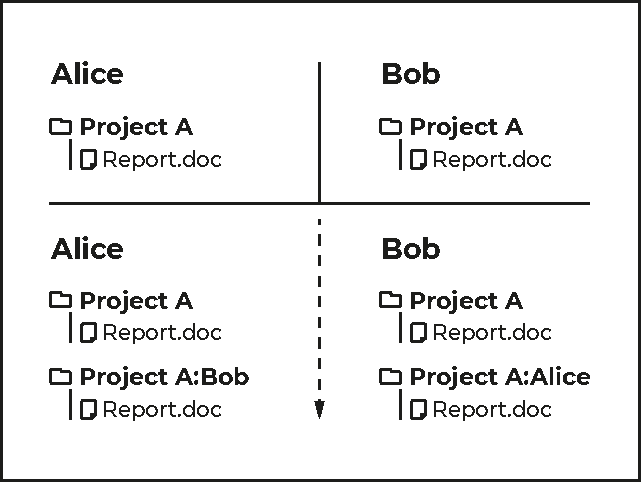
\includegraphics[scale=0.5]{AliceBob-font-des-fichiers.pdf}
\end{figure}

\subsubsection{Name conflict resolution in ElmerFS}

To distinguish between two inodes sharing the same name under the same parent directory, we use an additional internal unique identifier, the ViewID.

Apart from being unique, there is no particular requirement for this identifier.
We chose to use the user id (uid) and we expect that a user won’t issue operations
from two different processes. Note that it is a simplistic choice, many application might
log in under the same user on a system, we chose this to be able to map the ViewID to
sensible name. A more robust system could use an unique id associated with the ElmerFS process and then add metadata
to map it back to a username for example.

Each time a user creates a link, as illustrated in Figure~\ref{fig:fqn},
the system stores the name and the ino of the link as well as the ViewID of the user that created it.
Entries that would have been previously considered the same (sharing the same name) are now distinct.

To interface with the user, we use the concept of partial and Fully Qualified Names (FQNs).
Partial names are how the user named the link, FQN are partial names concatenated with the ViewID.

At any time, the user can chose to refer to its file from the partial name or the FQN.

Since the ViewID is unique, we know that all visible links are uniquely identifiable.
Because we cannot show duplicate names under a folder, when a conflict has occurred we do not display the partial names
but the FQNs of the conflicting files. Otherwise, the system behaves as a local file system, only showing the original file names.

To prevent applications that do not expect files to be renamed. When there is a conflict, if a request only use a partial name, we always favor the ViewID of the requester. If the application's file is subject to a conflict, the application will
still be able to refer to its file directly without interruption.

Comparing to have a system that renames files, we always preserve the original name, when conflict happens, the application can still function without worrying of external updates. Intuitively, the user can always see its own file as untouched by the underlying system.

As a drawback, inodes can be queried in two ways at all time, which departs from the POSIX standard. Additionally, it adds the risk
that two applications thinks to work on the same inode where in fact they are not. This can occurs for applications that unconditionally create a file
expecting that one of the creation request will fail.

\begin{figure}[h]
	\caption{An example of the name resolution in ElmerFS. The set above is
	what the folder contains.}
	\label{fig:fqn}
	\Description{A folder contains two conflicting entries with similar names.
	             The user is able to query its folder using a partial name or
				 the one in conflict using the fully qualified name.}
	\centering
	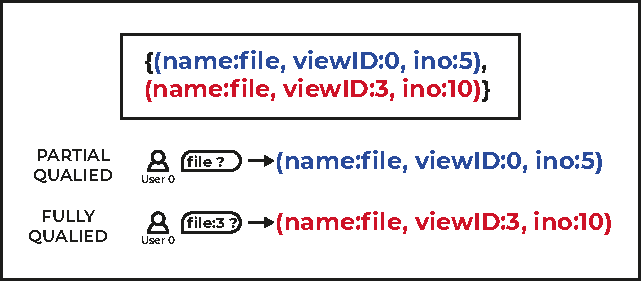
\includegraphics[scale=0.6]{Le-bonhomme-sait-pas-ce-quil-veut.pdf}
\end{figure}


\subsection{Divergent renames}

As explained in Section~\ref{fs:weak}, without coordination, \textit{rename} can not only create
cycles but also additional links.

Using a counter to track the number of links is no longer sufficient because at the time we issue
the \textit{rename} operation we cannot know if the operation will end up being concurrent. We
risk wrongly count the number of links and deleting an inode prematurely.

We use another RWSet that is always updated in the same transactions (\S~\ref{sec:transaction_layer}) that create or remove
a directory entry.

Each link contains the parent inode number and the FQN that contains the ViewID.
We use the ViewID again to have the exact same semantics as the set storing
the directory entries. Thus the link set is always valid with respect to
links currently visible in the FS.

However, POSIX forbids directory to have multiple links. While we have the correct set of link
for our inode, we also need to ensure that even after a divergent rename, only one link of the
directory will stay visible.

An additional LWWR is used as an arbitrator to decide which link is valid. The LWWR is updated inside
the \textit{rename}'s transaction (\S~\ref{sec:transaction_layer}) and stores the parent inode number.

When ElmerFS loads a directory entry, it first check that the LWWR stored parent correspond to
the directory being looked up. If they do not correspond, the entry is removed and the file system
correctly inform the user that the entry does not exists. The drawback is that we may never reclaim
the entry with the wrong parent if the parent is never looked up.

\section{Conclusion}

In this paper, we explore the challenges in the design of a truly
concurrent shared geo-replicated file systems under weak consistency.

We propose ElmerFS, a CRDT-based file system.
ElmerFS ensures file system replicas eventually converge to a common,
correct state in the present of conflicting operations.
Conflict resolution in ElmerFS is designed with the aim of
not resulting in unexpected results.
We argue that this enables users to complement or reverse the results of conflict resolution
through traditional file system operations.

We have implemented a prototype of ElmerFS and are in the process of performing
experimental evaluation.

While there remain open problems to be addressed,
we believe that leveraging the properties of CRDTs is a promising path towards
highly available and truly concurrent file systems and believe that future
work should go in this direction.

\section{Discussion}

In this section, we introduce directions for further research and open questions that
we would welcome feedback on:

\begin{itemize}
    \item \textbf{Cycles with concurrent renames}
    Our implicit hierarchy using map CRDTs does not prevent the creation of cycles.
    CRDT tree designs have been proposed~\cite{martin2012abstract}\cite{ahmed2012file}, but rely on multiple correction
    layers that perform additional operations to recover from broken invariants.
    We believe that both these issues could be solved by the use of post-conditions on merging
    concurrent updates.
    The key idea would be to merge operations only if the resulting state satisfies a given condition.
    For cycles, this would condition would be be that the resulting tree does not have a cycle~\cite{nair:hal-03150817}.
    Transactions that do not satisfy this condition would be discarded in a deterministic manner to ensure convergence.

    \item \textbf{Dealing with Orphan CRDTs}
    Our deletion strategy relies solely on issuing a delete operation for all
    known CRDTs of an entity.

    For file content, where we store an implicit and unbounded number of CRDTs,
    concurrent add operations conflict resolution can lead to content lingering
    without an entity to reference it.

    Tombstones are sometimes used in CRDT design, but here we need a mechanism to link and propagate deletion across multiple CRDT.

    We are not aware of any protocol that allows this. A possible framework could rely on a unique tombstone and use conditional
    transactions described in the previous section, ignoring the incoming operation from the various CRDT if the tombstone is set.

    \item \textbf{On performance and scaling}: We are conducting performance and scaling evaluation of ElmerFS.
    Our initial results show that ElmerFS lacks optimizations that more mature file system implement to achieve high throughput.
    We currently only implement write gathering and we would like to explore the behavior of our distributed file system in larger scale to support enterprise level workloads.

    \item \textbf{On conflict resolution for other operations}: We have not explored all possible conflict in ElmerFS yet.
    Permissions in weakly consistent systems are challenging~\cite{yanakieva2021access}.
    Cycles through rename operation are still possible due to our implicit tree representation.
    We would like to test specialized CRDT that prevent such occurrences while still allowing our current behavior. Recent work on tree CRDT might be a good fit~\cite{nair:hal-03150817}.
\end{itemize}


% // Commenting this because there is a paper about that (the one Marc sent us)
% // Design and Implementation of a Concurrency Benchmark Tool for Cloud Storage Systems
% \textbf{On tests}: We have tested ElmerFS with some classic test tools designed for local file system. Distributed file systems involve additional considerations for testing, not covered by those tools. We have performed ad-hoc conflict resolution tests, however we believe that it should be possible to automate this process with a tool that exhaustively tests all pairs of possible operations to ensure that the file system always converge to an expected state.


\bibliographystyle{ACM-Reference-Format}
\bibliography{elmerpap}

\end{document}
